\documentclass{article}
\usepackage[T1]{fontenc}
\usepackage[utf8]{inputenc}
\usepackage{graphicx}
\graphicspath{ {./images/} }
\usepackage[french]{babel}
\usepackage{xcolor}
\usepackage{listings}
\usepackage{hyperref}
\usepackage{fancyhdr}
\usepackage{tikz}
\usepackage{float}

\lstset {
    %language=Scheme,%il connait, ni scheme ni racket
    frame=tb,
    tabsize=4,
    showstringspaces=false,
    numbers=left,
    %upquote=true,
    commentstyle=\color{commentgreen},
    %keywordstyle=\color{eminence},
    stringstyle=\color{red},
    basicstyle=\small\ttfamily\color{blue}, % basic font setting
    emph={int,char,double,float,unsigned,void,bool},
    emphstyle={\color{blue}},
    escapechar=\&,
    % keyword highlighting
    classoffset=1, % starting new class
    otherkeywords={>,<,.,;,-,!,=,~},
    morekeywords={>,<,.,;,-,!,=,~,\&},
    %keywordstyle=\color{weborange},
    classoffset=0,
}

\usepackage{geometry} %marges
\geometry{left=3.5cm, right=3cm}

% « » 
\title{Rapport de projet Racket : Actor Shooting Star}
\author{Auteurs : Boudroua Imad, Gauchet Augustin, Nguyen Olivier, Zghari Hicham \\ Equipe 9145 \\ Encadrants : M.Renault et M.Rollet}
\begin{document}

\label{debut}
\thispagestyle{empty}
\begin{figure}%[ht]

\includegraphics[scale=0.6]{logo.jpg}
\end{figure}

\label{sommaire}

\begin{center}
\begin{tikzpicture}
\node[align=center,draw,thick,minimum width=\textwidth,inner sep=6mm] (titlebox)%
{\textsc{\textbf{\huge S6}}\\[\baselineskip]\textsc{\ }\\[\baselineskip]\textbf{\Huge Acting Shooting Star}\textsc{\ }\\[\baselineskip]};
\node[fill=white] (W) at (titlebox.north) {\bfseries \huge Projet};
\node (feat) at ([yshift=-9mm]titlebox.south){\bfseries \Large Boudroua Imad \ \ \ Zghari Hicham};
\node (feat) at ([yshift=-18mm]titlebox.south){\bfseries \Large \ Nguyen Olivier \ \ \ Gauchet Augustin};
\node (feat) at ([yshift=-27mm]titlebox.south){\bfseries \Large Equipe 9145};
\node (feat) at ([yshift=-60mm]titlebox.south){\bfseries \Large \ Encadrants : M.Renault et M.Rollet};
\end{tikzpicture}
\end{center}

\newpage

\pagestyle{fancy}
\fancyhf{}
\lfoot{Equipe 9145}%si vous voulez enlever le titre en bas de page enlevez ca
\rfoot{Page \thepage/\pageref{LastPage}}
\renewcommand{\headrulewidth}{0pt}
\renewcommand{\footrulewidth}{0pt}

%\maketitle
%
\includegraphics[width=\textwidth]{logo.jpg}
%\newpage
\tableofcontents
\newpage

\section{Introduction et analyse du projet}
\subsection{Contexte}
Dans le cadre du second projet de programmation en première année d'informatique à l'ENSEIRB-MATMECA, nous avons eu à prendre pour exemple le jeu \textbf{Acting Shooting Star}, en langage \textbf{Racket}. Ce rapport va permettre d'expliquer les démarches que notre groupe a effectuées pour mener ce projet.

\subsection{Problématique}
Le but de ce projet est d'implémenter le modèle de l'acteur : un monde rempli d'acteurs intervenant par le biais de messages. L'enjeu est alors d'assurer l'interaction entre les acteurs, c'est à dire implémenter leur comportement selon la réception de messages, leur permettre d'en envoyer aux autres et de pouvoir en créer de nouveaux.


\subsection{Cadre de travail}
À cause de la pandémie de Coronavirus, nous avons dû travailler chez nous, certains en ssh et d'autres en machines virtuelles. Les différences de configuration et le manque de maîtrise du ssh ont notamment été un frein au développement du projet. Le code a dû également subir de nombreuses restructurations pour plus de clarté.

\subsection{Bibliothèques utilisées}
%Les bibliothèques que nous avons utilisé dans le cadre du projet sont:

\begin{enumerate}
\item \textcolor{red}{Raart:} fournit un modèle algébrique d'ASCII qui peut être utilisé pour l'art, l'interface utilisateur et les diagrammes. Dans notre projet, il a été utilisé essentiellement pour mettre le jeu dans un cadre déterminé par quatre variables ($x_1$,$x_2$,$y_1$,$y_2$) et dans l'affichage des joueurs avec les différents symboles et couleurs.
\item \textcolor{red}{Lux:} fournit un moyen efficace pour la création des programmes qui interagissent en temps réel avec l'utilisateur.
\item\textcolor{red}{Rackunit:} est une bibliothèque facilitant la mise en place de tests afin de s'assurer du bon fonctionnement du code.

\end{enumerate}
%(struct actor (position mailbox name category)) \\
%La structure actor est au coeur du projet, elle permet la création du %joueur, d'ennemis ou encore de projectiles. Elle est composée d'un %champ position (liste de 2 éléments x et y), d'un champ mailbox %(contient une liste de message que l'acteur doit exéctuer), d'un %champ name qui correspond à la représentation ASCII de l'acteur et %category (joueur, ennemi, projectile).

\section{Fonctionnalités développées}

Afin d'assurer les interactions entre les acteurs, nous avons non seulement implémenté la structure de données \textbf{actor}, mais aussi d'autres structures qui régissent leur fonctionnement. Les acteurs sont regroupés dans une structure \textbf{world}, et la structure \textbf{runtime} permet de les manipuler en leur envoyant des messages à chaque \textbf{tick} de jeu.

\subsection{Actor}

\subsubsection{Structure et mise à jour des acteurs}
La structure \textbf{actor} est au coeur du projet, elle permet la création du joueur, d'ennemis ou encore de projectiles. Elle est composée de quatre champs:

 \definecolor{monVert}{rgb}{0.,0.4,0.0} 
 
\begin{itemize}
    \item \textbf{position} est une liste de deux éléments qui contient les coordonnées $x$ et $y$
    \item \textbf{mailbox} est une liste de messages
    \item \textbf{name} contient la représentation visuelle en \textbf{raart} de l’acteur
    \item \textbf{category} est le type de l’acteur (\textbf{player}, \textbf{enemy}, \textbf{projectile})
\end{itemize}

Pour faire fonctionner ce projet, il est nécessaire de pouvoir mettre à jour les coordonnées d'un acteur ou d'en créer de nouveaux en accord avec sa \textbf{mailbox}. Pour ce faire nous avons implémenté la fonction \textcolor{blue}{\lstinline{actor-update}}.

Cette fonction parcourt récursivement la \textbf{mailbox} en effectuant les instructions situées dans les messages au fur et à mesure de son exécution. Sa complexité en temps est donc linéaire en fonction de la longueur de sa \textbf{mailbox}. De plus, cette fonction est récursive terminale, ce qui permet à l'interpréteur de l'optimiser.

\subsubsection{Gestion des collisions}
Afin de détecter les collisions entre les acteurs, nous avons comparé positions relatives des acteurs à chaque tick de l'horloge. Pour cela, la fonction \lstinline{colliding?} a été implémentée pour vérifier si deux acteurs sont entrés en collision. La fonction \lstinline{collisions?} nous permet de savoir s'il y a eu des collisions entre les différents acteurs. Elle est de complexité linéaire en fonction du nombre d'acteurs.

\subsection{World}

\subsubsection{Structures et fonctions}

La structure \textbf{world} est constituée d'une liste regroupant tous les acteurs. Elle assure l'interdépendance entre les acteurs et permet leur actualisation et leur interaction par la fonction \lstinline{update-word}. Le monde agit sur les acteurs mais les acteurs peuvent aussi interagir sur celui-ci par le biais de fonctions comme \lstinline{send-to-world} qui envoie un message à tous les acteurs du \textbf{world}. Ainsi, le monde permet de se détacher d'une vision individualiste d'un acteur qui évolue et s'actualise seul et d'arriver à une interdépendance entre les différentes entités qui évoluent. Les fonctions les plus importantes sont celles ci-dessous : 

\begin{itemize}
    \item \lstinline{world-update} est au coeur du projet puisqu'elle permet la mise à jour de tous les acteurs du \textbf{world}. Pour ce faire, elle appelle la fonction \lstinline{actor-update} pour chaque acteur de la liste, ce qui signifie une complexité en temps linéaire en fonction du produit du nombre d'acteurs présents par la longueur de \textbf{mailbox}.
    \item \lstinline{generate} est une fonction qui permet de générer aléatoirement de nouveaux acteurs pour le jeu et de les ajouter au \textbf{world}
    \item \lstinline{game} est la fonction qui régit chaque \textbf{tick} du jeu. Elle sauvegarde le \textbf{world} (cf partie suivante), élimine les acteurs qui sont entrés en collision et génère les ennemis.

\end{itemize}

\subsubsection{Retour dans le temps} 

Nous avons mis en place une fonction pour revenir en arrière dans notre jeu. Pour ce faire nous avons utilisé une liste \textbf{latest-worlds} déclarée en variable globale dans notre fichier qui contient comme son nom l'indique les dernières structures \textbf{world} actualisées. Elles sont classées de la plus récente à la plus ancienne. 

À chaque tour de boucle du jeu, une copie du \textbf{world} actuel est ajoutée dans \textbf{latest-world} par la fonction \textcolor{blue}{\lstinline{save-world}}. Cette fonction ajoute en tête de liste le world à sauvegarder et dans le cas où la liste est de taille supérieure à 20, elle supprime le dernier élément de la liste quand elle ajoute un élément. Effacer le dernier élément de la liste consiste à inverser la liste, prendre son \lstinline{cdr} et l'inverser encore une fois, \textcolor{blue}{\lstinline{save-world}} est alors de complexité quadratique par rapport à la taille de la liste dans le pire des cas. Néanmoins la liste est de taille $20$ au maximum.

Pour revenir en arrière de $n$ ticks il suffit de remplacer le \textbf{world} actuel par le n-ième élément de \textbf{latest-worlds}, c'est ce que fait la fonction \textcolor{blue}{\lstinline{world-travel}} qui est ainsi récursive terminale de complexité linéaire par rapport à la n (nombre de ticks à revenir en arrière). De manière pratique (principalement pour débugguer), nous avons permis au joueur de revenir de 15 ticks en arrière lorsqu'il appuie sur "p".

L'implémentation d'une liste en variable globale aurait pu être évitée en intégrant une liste de \textbf{world} dans la structure représentant la boucle de jeu. Nous y avons pensé trop tard et si nous avions eu plus de temps, nous aurions opéré le changement.

\subsection{Runtime}
\textbf{runtime} est une structure qui orchestre le jeu entre les acteurs. D'une part, elle contrôle l'écoulement du temps et la durée du jeu et d'autre part elle organise la transmission des messages et les traduit en événements. Son utilisation avec la bibliothèque  \textcolor{red}{Lux} a permis d'interagir avec les entrées du clavier. Cela s'avère utile en ce qui concerne le contrôle du jeu par un utilisateur. L'implémentation de cette structure s'articule autour de 4 éléments principaux :

\begin{enumerate}
\item \textbf{world-fps} initialise le nombre d'images par seconde que le jeu est censé s'afficher.  
\item \textbf{world-event} gère les événements qui se produisent et les interactions avec les périphériques extérieurs.
 \item \textbf{world-output} permet d'afficher les éléments de la bibliothèque \textcolor{red}{raart} sur le terminal.  
 \item \textbf{world-tick} s'occupe de mettre à jour la nouvelle \textbf{runtime} après chaque unité de temps.

\end{enumerate}

\subsection{Documentation}
Nous avons écrit notre documentation avec Scribble. Elle contient l'explication détaillée des structures et fonctions utilisées. L'utilisation des fonctions \textcolor{blue}{\lstinline{defproc}} et \textcolor{blue}{\lstinline{defstruct}} permet d'établir rapidement une documentation structurée.

%\section{Choix de l'implémentation}
%\subsection{Déviation de la programmation fonctionnelle}
%\subsubsection{Retour dans le temps}

\section{Tests employés et contrats}
Les tests consistent principalement à vérifier que les fonctions renvoient bien ce qu'elles sont sensées renvoyer, ils nous ont permis de nous donner de la confiance dans notre code. Par exemple, pour tester \textcolor{blue}{\lstinline{actor-update}}, nous avons appliqué la fonction à divers acteurs possédant une \textbf{mailbox} différente. Nous avons ensuite vérifié que les résultats obtenus coïncidaient avec ceux escomptés. Certains tests ont néanmoins nécessité un affichage pour s'assurer que leur implémentation n'était pas défectueuse, notamment \textcolor{blue}{\lstinline{world-travel}} et la fonction qui génère les projectiles.
\newline
Un exemple de test consiste à contrôler les renvois de la fonction \lstinline{actor-update} en se mettant en condition de chaque cas du \textbf{cond}. On vérifie ensuite que les fonctions renvoient les bons résultats attendus pour chaque test portant sur ces conditions. 

Dans l'optique de vérifier que nos fonctions se comportent comme prévu, nous avons également fait des contrats. Ces contrats nous assurent que les fonctions sont appelées avec les bons types de paramètres, et qu'elles renvoient le bon type de données. Ils permettent ainsi de rendre notre code plus sûr.

\section{Conclusion}
Le jeu codé est un shooter simple où le but est de survivre tout en éliminant le plus d'ennemis possibles. Le joueur possède une unique vie et meurt lorsqu'il heurte un mur ou un ennemi.
\begin{figure}[H]
    \centering
    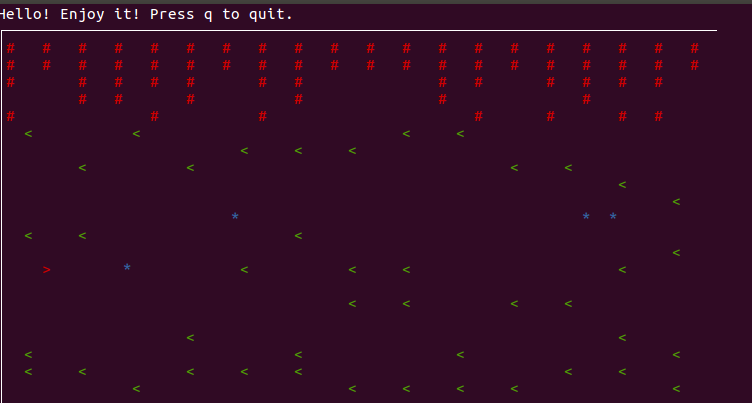
\includegraphics[width = 12cm]{jeu.png}
    \caption{Capture d'écran du jeu}
    \label{Screenshot}
\end{figure}
Le projet de programmation fonctionnelle nous a ainsi permis de nous détacher de la programmation impérative. En effet, nous avons découvert un nouveau modèle de programmation qui consiste à n'utiliser que le résultat d'application des fonctions ce qui assure la transparence référentielle. Nous avons aussi intégré la notion du typage dynamique qui diffère du typage statique auquel nous étions habitués.
\label{LastPage}
\end{document}t\textit{}
